\documentclass{report}
\usepackage[utf8]{inputenc}
\usepackage[romanian]{babel}
\usepackage{float}
\usepackage{graphics}
\usepackage{graphicx}
\title{Programare WEB \\ Documenta\c tie \\ Grading Script App}
\author{Botescu Mihai: \texttt{mihai.botescu00@e-uvt.ro} \\ Beze Robert: \texttt{robert.beze00@e-uvt.ro}}
\date{\today}

\begin{document}

\maketitle
\begin{abstract}
    Aplicatia presupune un script pentru notele studentilor obtinute la diferite materii pe parcursul semestrului cat si la examen. 
Aplicatia va fi utilizata atat de profesori cat si de studenti. Accesul la aplicatie se va realiza pe baza autentificarii cu credentialele conturilor de e-uvt, prin email-ul institu\c tional. 
\end{abstract}
\tableofcontents
\chapter{Introducere}
\section{Definirea problemei}
Din perspectiva studentului, acesta acceseaza platforma, se autentifica folosind credentialele. Este prezent un meniu cu mai multe optiuni (materiile la care acesta este inscris). Studentul  selecteaza o materie, si este redirectionat la o pagina care expune 3 meniuri: notele la componentele de la curs, notele de la componentele de la laborator, nota finala.
Din perspectiva profesorului, acesta detine un meniu pt fiecare materie predata; pentru fiecare meniu, un dropdown list cu studentii inscrisi la acel curs.
 
\section{Resursele aplica\c tiei}

\subsection{Stabilirea resurselor}
Resursele \cite{Masse2011} stabilite la nivel de aplica\c tie sunt urm\u atoarele:

\begin{itemize}\item Materia (materiile; colectie) resursa principala  \begin{itemize} 
\item Nota (notele; colectie) 
\item Prezenta (prezentele; colectie -> pentru fiecare Curs, Seminar/Laborator in parte) 
\end{itemize} \item Utilizatorul (student/profesor) resursa principala \begin{itemize}
\item Profesor (singleton) 
\item Studentul (sau studentii – colectie) 
\end{itemize}
\end{itemize}

\newpage 

\subsection{Opera\c tii pe resursele vizate in aplica\c tie}

Figura \ref{swagger_ops} sugerează opera\c tiile \cite{Masse2011} realizate pe fiecare dintre resurse în parte:

\begin{figure}[h!]
    \centering
    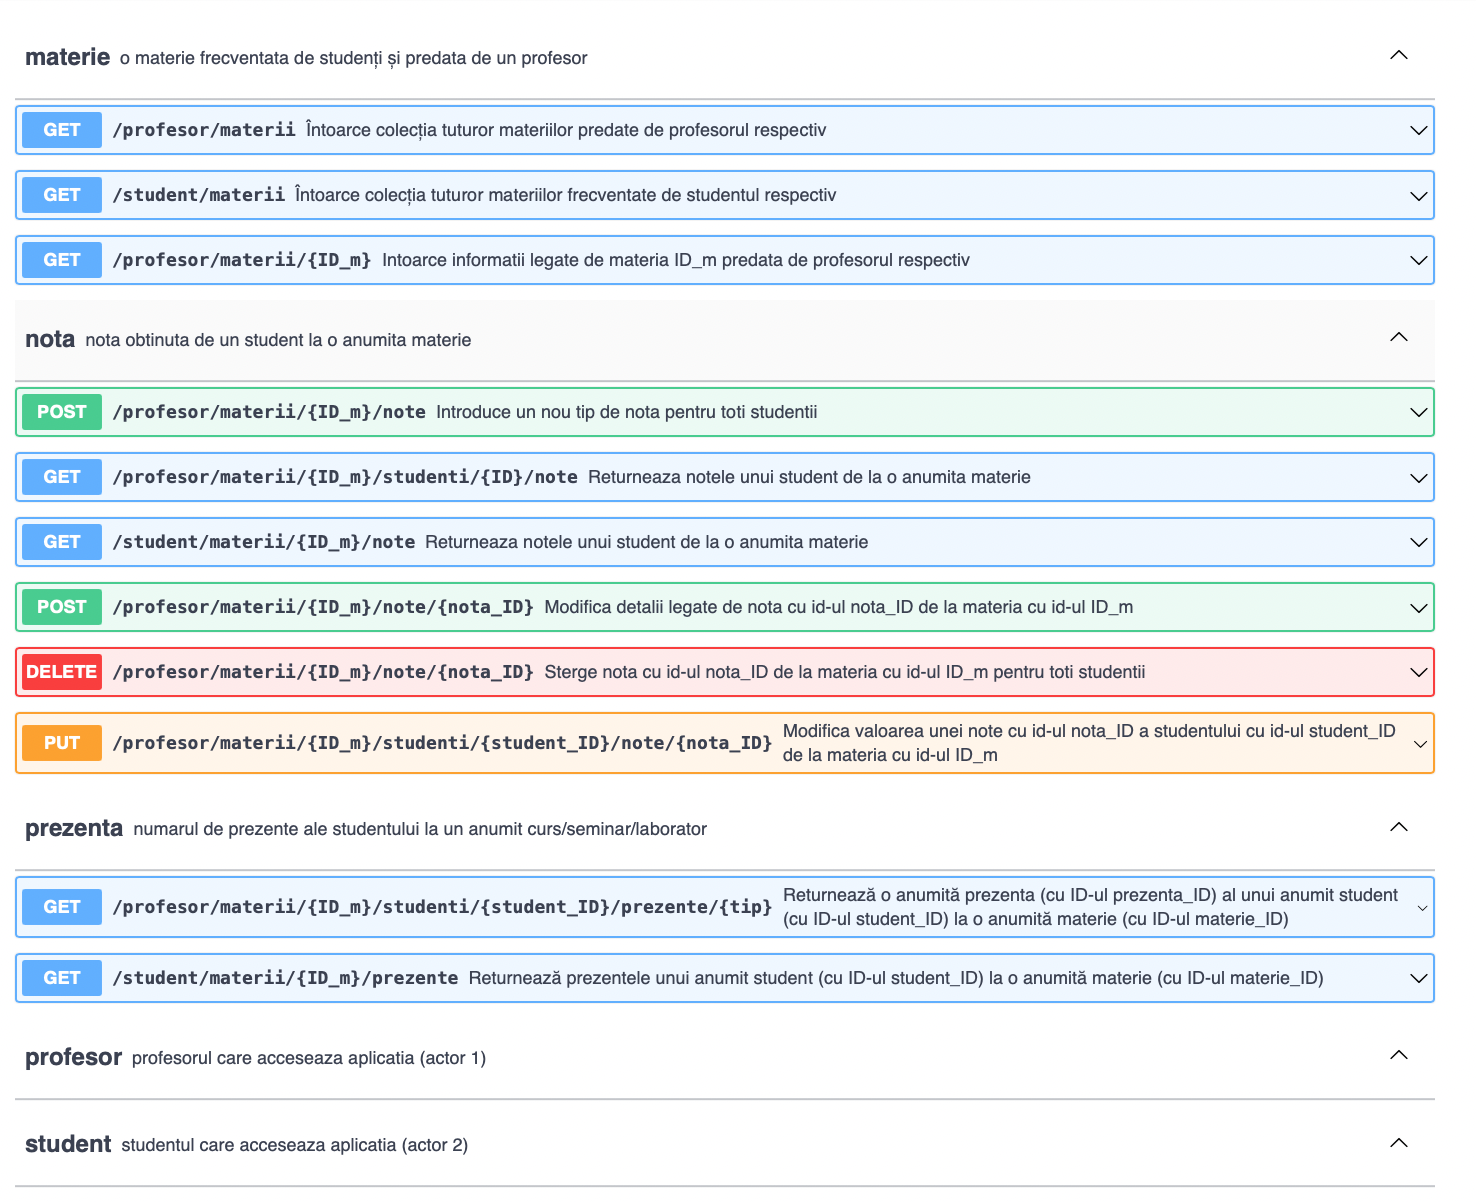
\includegraphics[width=300pt]{img/swagger_ops.png}
    \caption{Opera\c tiile pe resursele vizate în aplica\c tie}
    \label{swagger_ops}
\end{figure}
\chapter{Ingineria sistemului}
\section{Arhitectura propusă}
Se va merge pe ideea de a utiliza modelul client-server, care să respecte constrângerile ReSTful \cite{Masse2011}. Mai precis, va avea loc separarea serviciilor de UI, prin intermediul API-ului. API-ul expune servicii care sunt consumate în UI.
Interac\c tiunea client - server va avea loc prin cereri tipice (de tip GET, POST, PUT, DELETE). Server-ul va emite client-ului, în urma unei cereri, un răspuns tipic (de regulă, în format JSON). Modele de cereri \c si răspunsuri din partea client-ului \c si a server-ului au fost ilustrate în Sprint-ul anterior, în momentul definirii \c si dezvoltării API-ului \cite{Vaswani2008-ms}.
Separat de comunicarea client-server, vor exista serviciile definite \c si implementate.
\section{Cazuri de utilizare ale aplica\c tiei}
Aplica\c tia va avea, la cel mai înalt nivel, din perspectiva utilizatorului \c si a modului de lucru cu aceasta, 2 principali actori (considera\c ti ca fiind de asemenea \c si resurse unitare): profesorul \c si studentul.
Astfel, identificăm 2 scenarii pe baza acestor actori: utilizare din perspectiva studentului, utilizare din perspectiva profesorului.
\subsection{Cazuri de utilizare din perspectiva studentului}
Diagrama de mai jos \ref{dgram1} reprezintă (sumar) etapele pe care le va parcurge studentul în utilizarea aplica\c tiei.

\begin{figure}[h!]
    \centering
    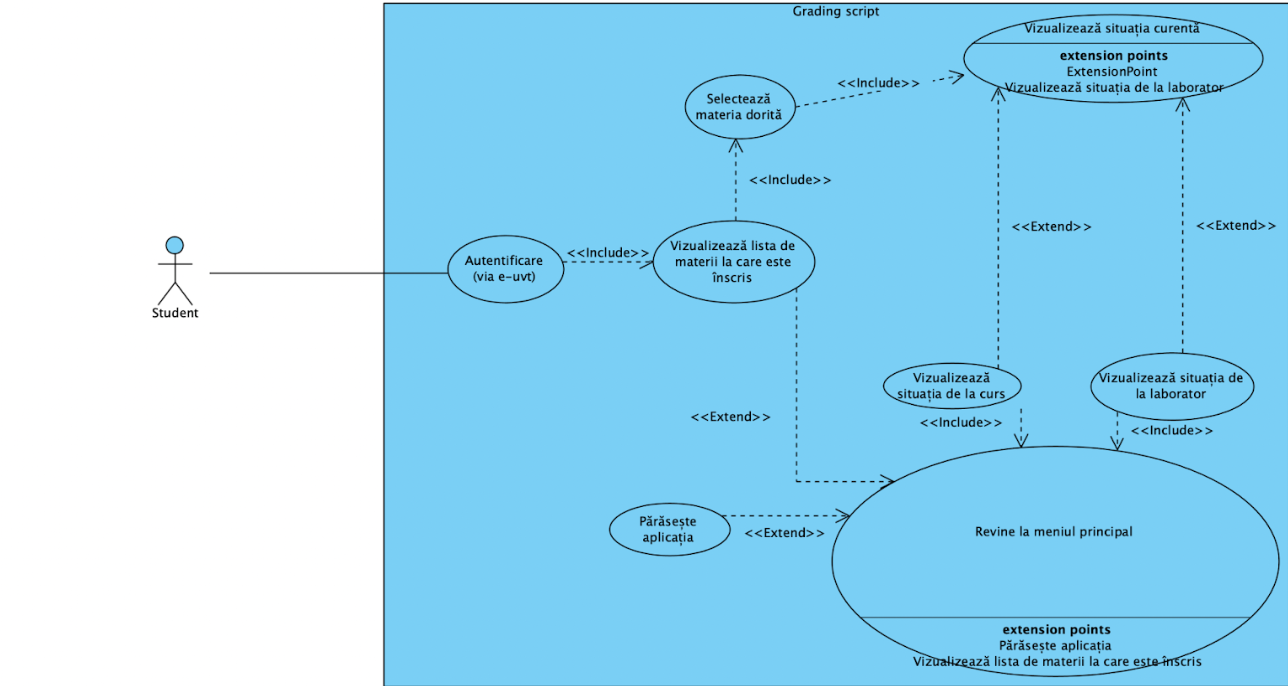
\includegraphics[width=300pt]{img/dgram1.png}
    \caption{Diagrama cazurilor de utilizare din perspectiva studentului}
    \label{dgram1}
\end{figure}

\subsection{Cazuri de utilizare din perspectiva profesorului}

Diagrama de mai jos \ref{dgram2} reprezintă (sumar) etapele pe care le va parcurge profesorul în utilizarea aplica\c tiei.

\begin{figure}[h!]
    \centering
    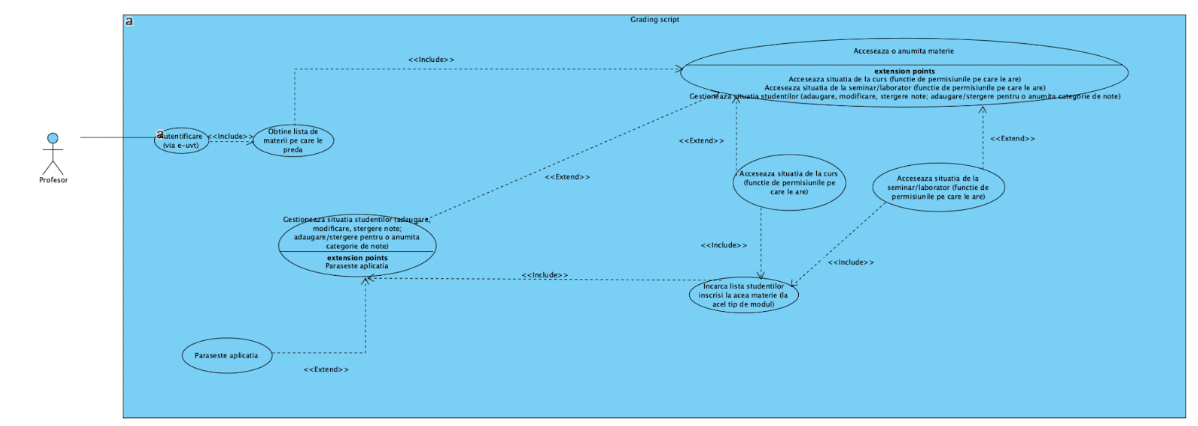
\includegraphics[width=300pt]{img/dgram2.png}
    \caption{Diagrama cazurilor de utilizare din perspectiva profesorului}
    \label{dgram2}
\end{figure}

\section{Schimburile de mesaje între utilizatorii aplica\c tiei}

Interac\c tiunile \c si schimburile de mesaje dintre actori au fost eviden\c tiate prin prisma definirii API-ului.

\section{Stocarea datelor}

Figura \ref{dbdgram} desemnează diagrama entitate-rela\c tie a bazei de date prin prisma căreia urmează să putem gestiona fluxul de date din aplica\c tia noastră.
De men\c tionat este că se vor utiliza 2 tipuri de baze de date: Maria DB (integrat în phpMyAdmin) \c si sqlite3 (integrat via fi\c sier local, parte din proiect).


\begin{figure}[h!]
    \centering
    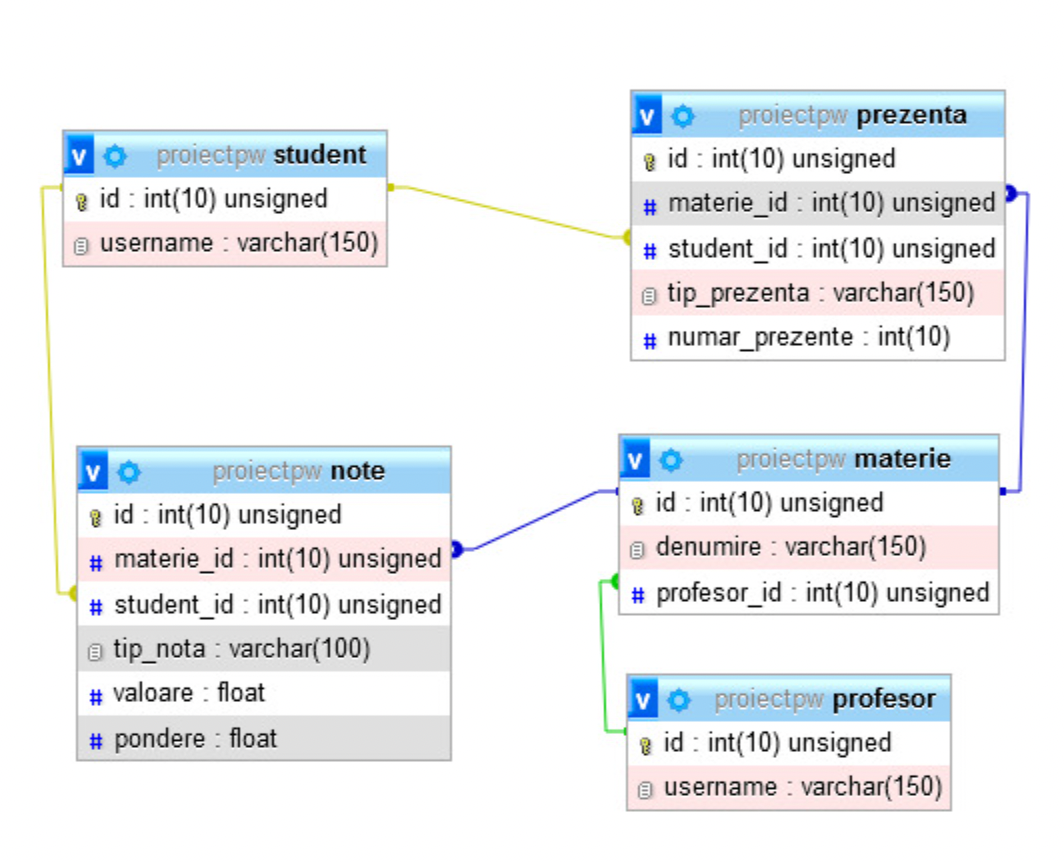
\includegraphics[width=300pt]{img/dbdgram.png}
    \caption{Diagrama entitate-rela\c tie reprezentând schema bazei de date utilizate}
    \label{dbdgram}
\end{figure}



La o materie există mai multe note, dar un anumit tip de notă poate apar\c tine unei singure materii (rela\c tie one-to-many). La o materie, există mai multe prezen\c te, dar un tip de prezen\c tă apar\c tine unei singure materii (rela\c tie one-to-many). La fel, un student are mai multe tipuri de prezen\c te, în timp ce, o prezen\c tă apar\c tine unui student (rela\c tie one-to-many). În cazul studentului, acesta poate ob\c tine mai multe tipuri de note, în timp ce, o notă apar\c tine unui student (rela\c tie one-to-many). Studentul \c si materia se află în rela\c tie many-to-many, fiindcă un student poate fi înscris la mai multe materii, \c si reciproc, o materie con\c tine o listă de studen\c ti înscri\c si la aceasta.
Au fost introduse \c si o varietate de constrângeri (constrângeri de cheie - primară, străină; constrângeri pentru valorile pe care le pot lua anumite câmpuri – de exemplu, nota este un număr real cu valori de la 1 la 10).
\newpage 

\section{Ingineria cerin\c telor}

\subsection{Cerin\c te pentru Sprint 2}

Prin intermediul MS Teams, s-au decis a fi abordate următoarele cerin\c te:

1. Modelarea frontend-ului - (cel pu\c tin 70-80\%) finalizat până la finalul sprint-ului 2

2. Implementarea unor elemente de interfa\c tă \c si a unor interac\c tiuni minimale

3. Proiectarea sistemului, ingineria sistemului, arhitectura acestuia

4. Dezvoltarea modelului bazei de date (integral: schema bazei de date, tabele, câmpuri, restric\c tii: chei primare, chei străine; restric\c tii asupra câmpurilor tabelelor)

5. Implementarea principalelor opera\c tii care să ofere o dezvoltare a cerin\c telor minimale: majoritatea opera\c tiilor de tip GET vor fi implementate până la finalul SPRINT-ului 2

6. Implementarea răspunsurilor pentru principalele opera\c tii care să ofere o dezvoltare a cerin\c telor minimale (operatii de get) – identic cu cerin\c ta anterioară, legat de deadline.

\subsection{Cerin\c te pentru Sprint 3}

Prin intermediul MS Teams, s-au decis a fi abordate următoarele cerin\c te:

1. Implementarea opera\c tiilor de modificare (rutele PUT, POST, DELETE)

2. Expunerea serviciilor pentru rutele PUT, POST, DELETE

3. Consumul serviciilor pentru rutele PUT, POST, DELETE

4. Finalizare front-end

5. Instalarea aplica\c tiei (configurarea selectării tipului bazei de date folosite: Maria DB sau sqlite3; popularea bazei de date cu câteva date minimale pentru ca aplica\c tia să fie utilizabilă \c si func\c tională)

\chapter{Tehnologii utilizate}

\section{Descrierea stivei de tehnologii}

\subsection{Front-end}

* HTML, CSS \cite{Duckett2011}, Bootstrap - pentru definirea \c si modelarea elementelor tipografice

* JQUERY \cite{York2015-ud} \cite{Rauschmayer2019-dk} (AJAX \cite{Ford2008-il}) - Apeluri asincrone, pentru a consuma serviciile expuse în API 

\subsection{Back-end}

* PHP \cite{Vaswani2008-ms} (v7), Slim 3, Twig: pentru rutarea paginilor, expunerea serviciilor

* PDO \cite{Vaswani2008-ms}: Nivelul de abstractizare utilizat pentru a putea comunica din aplica\c tie cu baza de date via query-uri

\subsection{Software utilizat}

MAMP (rulare server local), PHPMYADMIN (interfa\c tă pentru DBMS), Sqlite Studio Browser (pentru a testa dacă datele sunt salvate corect în baza de date sqlite), ReSTer (extensie Google pentru testare ReST), Postman (program pentru testare ReST), Composer (pentru a instala dependin\c tele necesare pentru o func\c tionalitate minimă pentru PHP).


\chapter{Testarea aplica\c tiei}

Ca \c si medii de testare ReST, s-au utilizat: cURL, ReSTer (extensie pentru web browser-ul Google Chrome) \c si Postman (aplica\c tie desktop).

\section{Cereri tip GET}

Testăm o cerere tip GET (în cazul de fa\c tă, studentul autentificat este \texttt{mihai.botescu00@e-uvt.ro}).

\texttt{GET /student/materii} returnează lista de materii frecventate de studentul autentificat, ca în exemplul din figura \ref{GET_CURL_OK}.

\begin{figure}[h!]
    \centering
    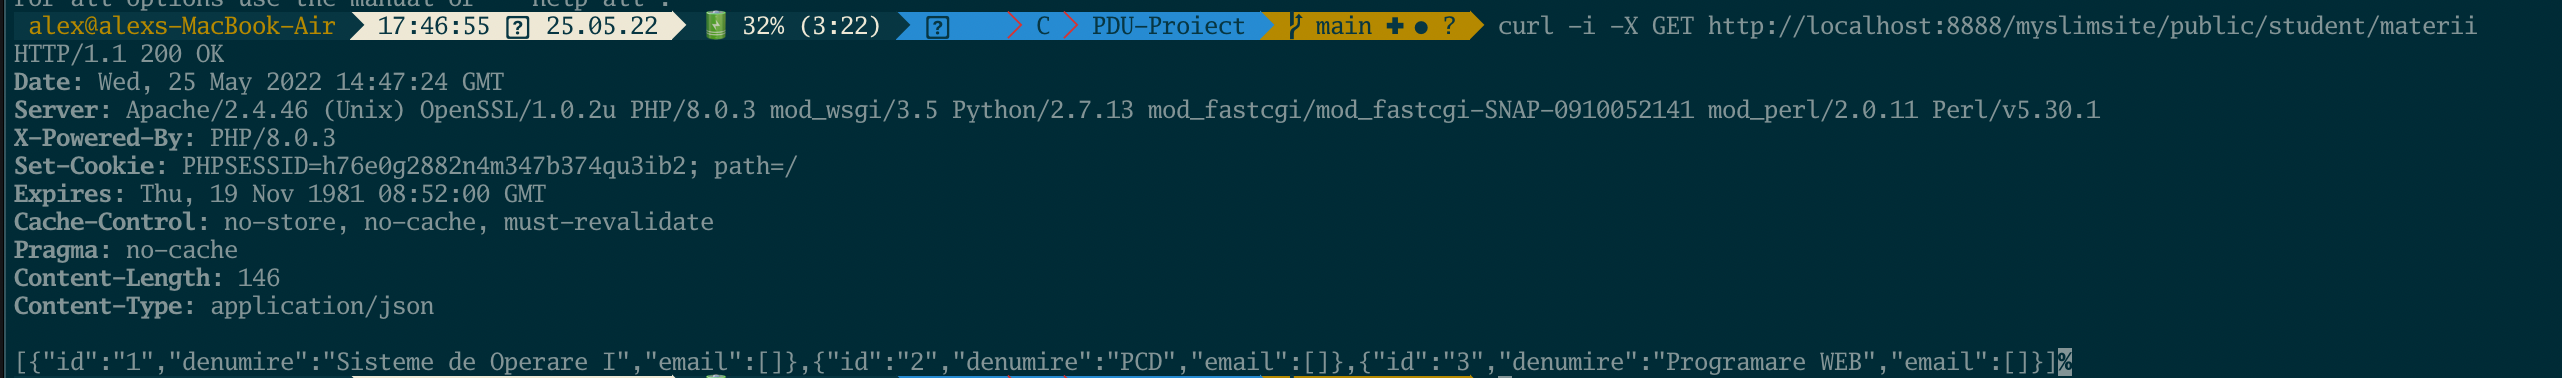
\includegraphics[width=300pt]{img/GET_OK_curl.png}
    \caption{Testare cerere GET via curl (success)}
    \label{GET_CURL_OK}
\end{figure}

\texttt{GET /profesor/materii} returnează lista de materii predate de profesorul autentificat, ca în exemplul din figura \ref{GET_CURL_ERR}. În cazul de fa\c tă, cum profesorul nu este autentificat, vom primi un mesaj de eroare.

\begin{figure}[h!]
    \centering
    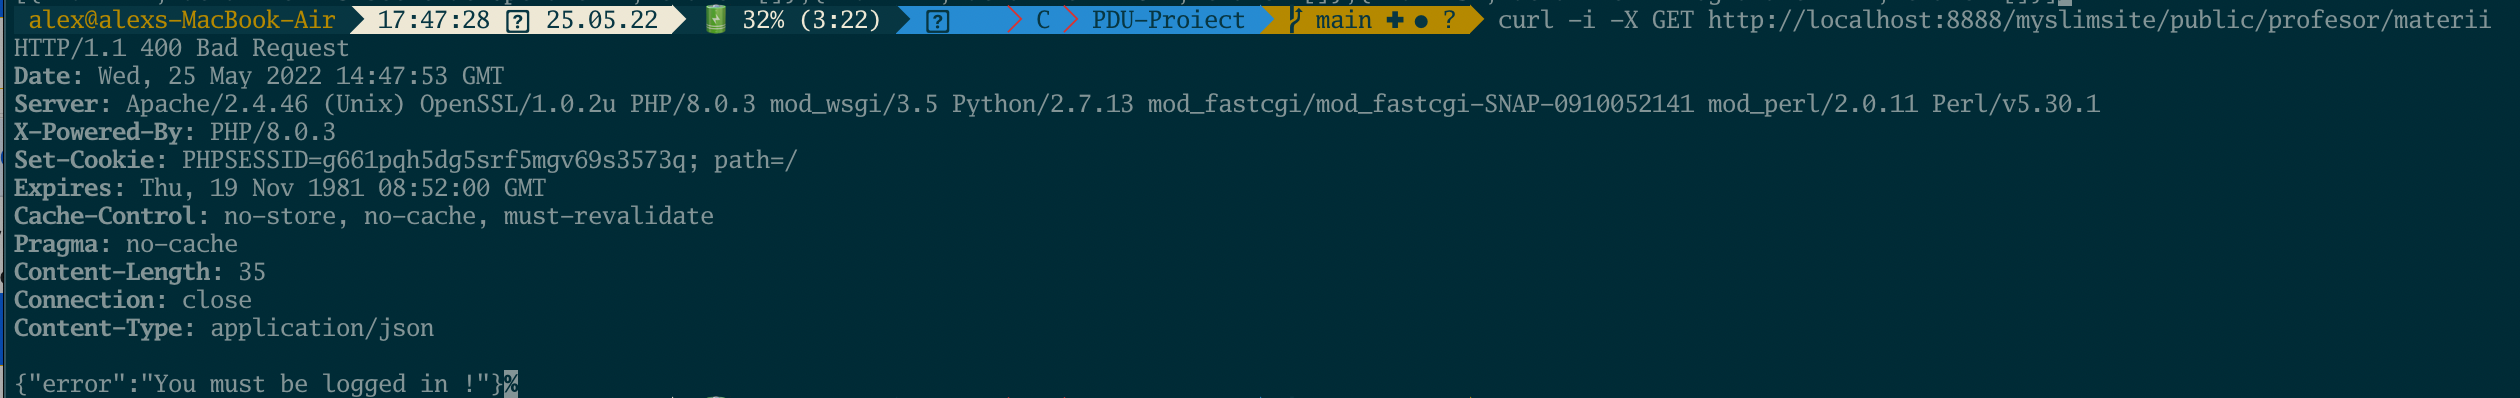
\includegraphics[width=300pt]{img/GET_ERR_curl.png}
    \caption{Testare cerere GET via curl (error)}
    \label{GET_CURL_ERR}
\end{figure}

\newpage 

\texttt{GET /student/materii/1/note} returnează notele studentului autentificat, de la materia cu ID-ul 1, ca în exemplul din figura \ref{GET_POSTMAN_OK}.

\begin{figure}[h!]
    \centering
    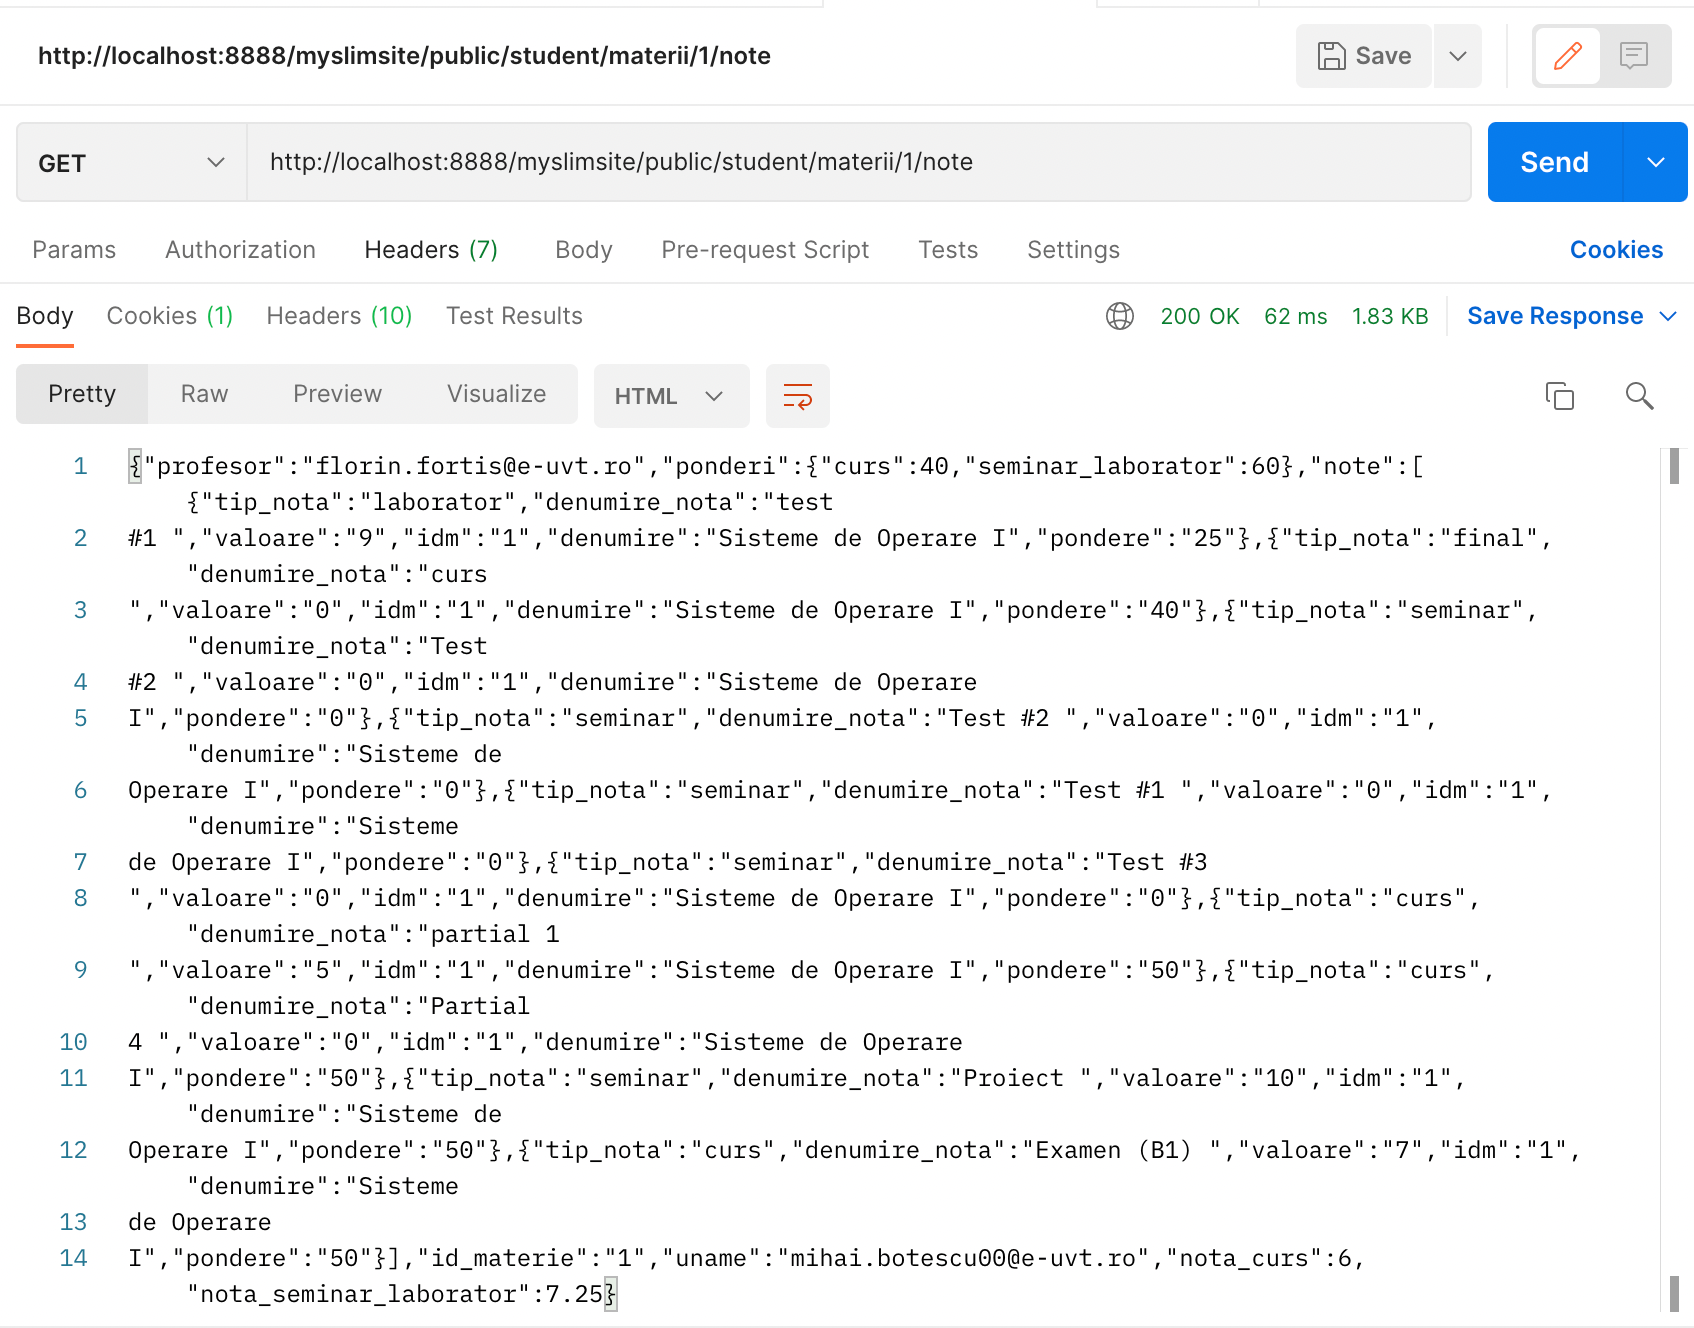
\includegraphics[width=300pt]{img/GET_OK1.png}
    \caption{Testare cerere GET via Postman (success)}
    \label{GET_POSTMAN_OK}
\end{figure}
\newpage 
\texttt{GET /profesor/materii/1/studenti/1/note} returnează notele studentului cu ID-ul 1, de la materia cu ID-ul 1, ca în exemplul din figura \ref{GET_POSTMAN_OK2}. Ne autentificăm cu profesorul, pentru ca extragerea datelor să fie posibilă.

\begin{figure}[h!]
    \centering
    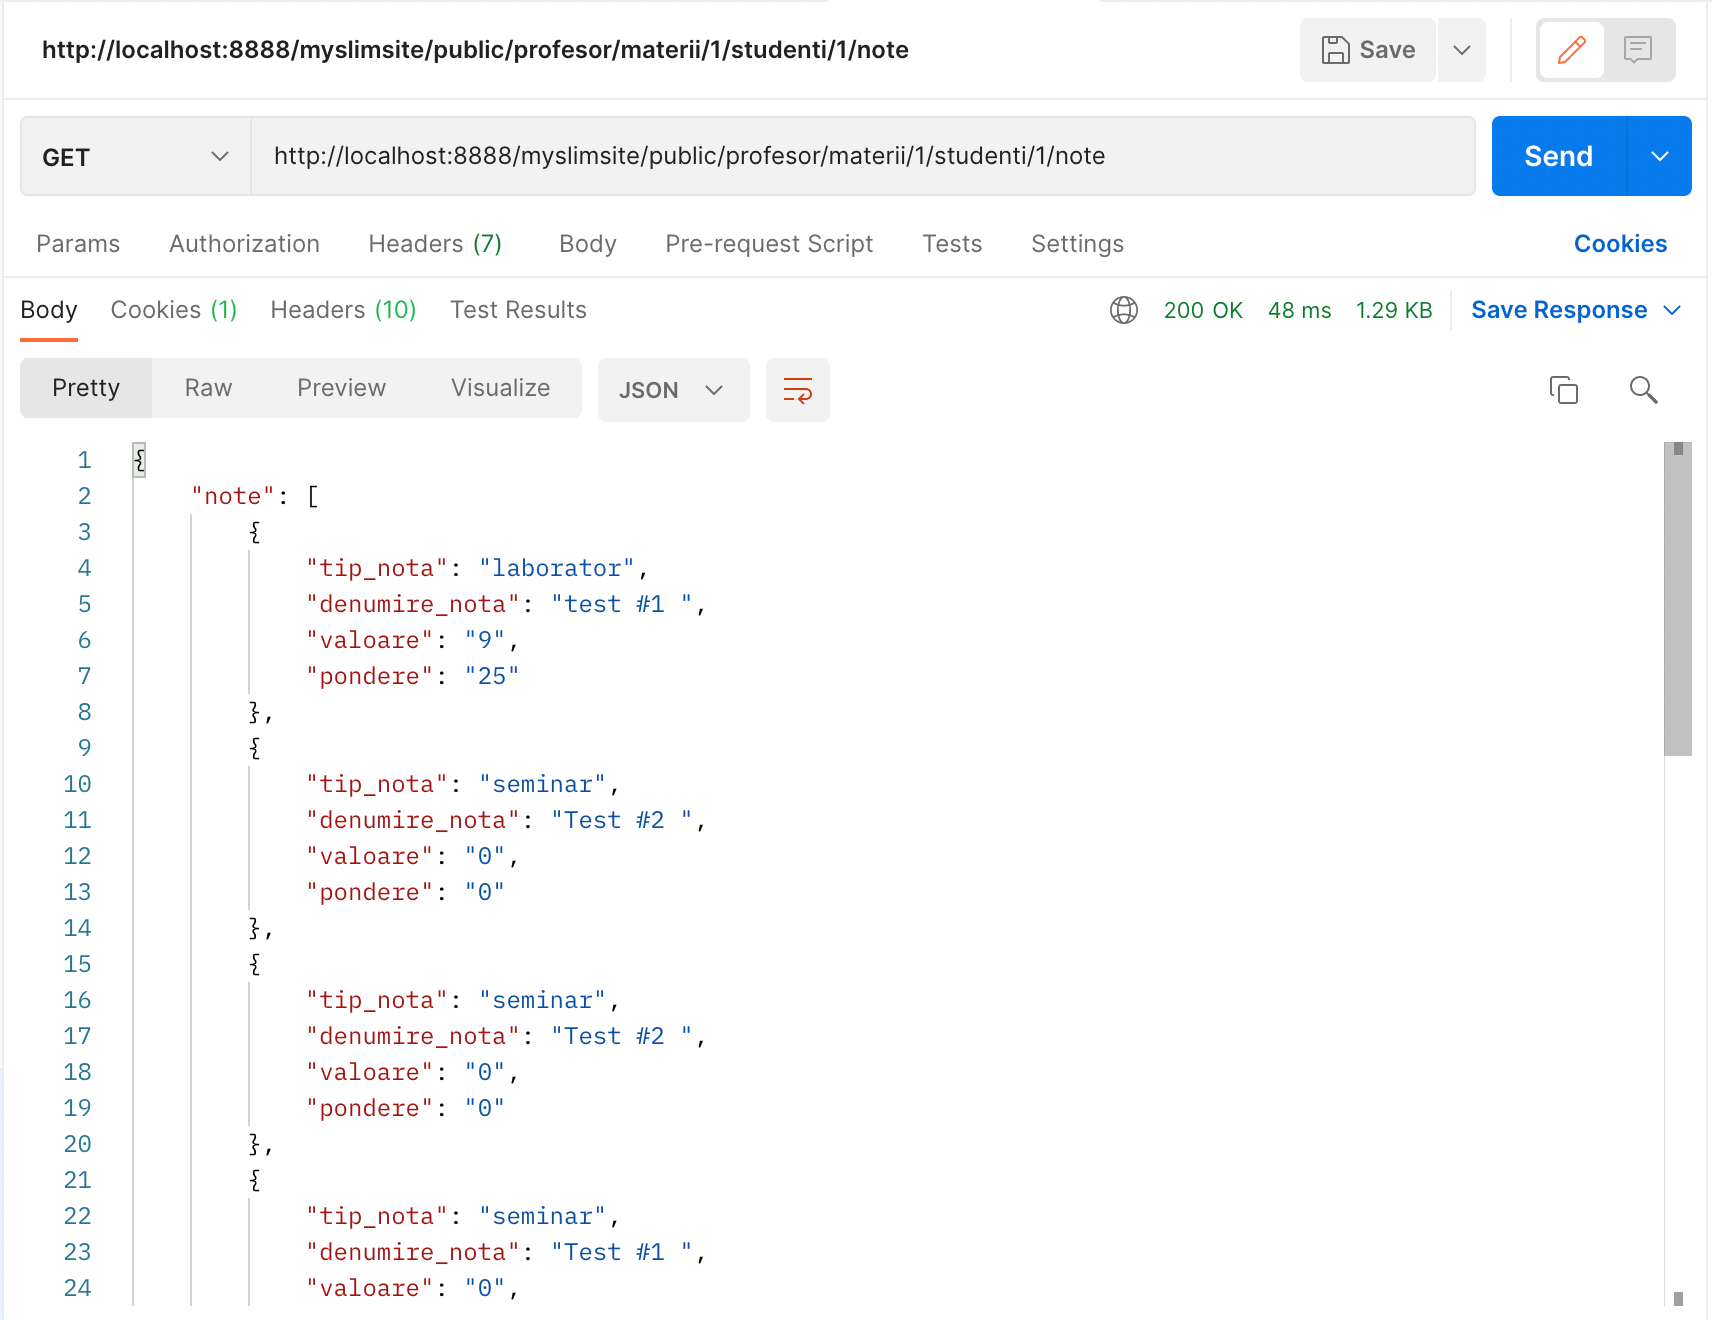
\includegraphics[width=300pt]{img/GET_OK.png}
    \caption{Testare cerere GET via Postman (success)}
    \label{GET_POSTMAN_OK2}
\end{figure}




\section{Cereri tip POST}

Adăugăm o notă nouă la o anumită materie, pentru profesorul autentificat curent.

De exemplu, pentru SO1, cum se vede în figura \ref{POST_OK}.

\begin{figure}[h!]
    \centering
    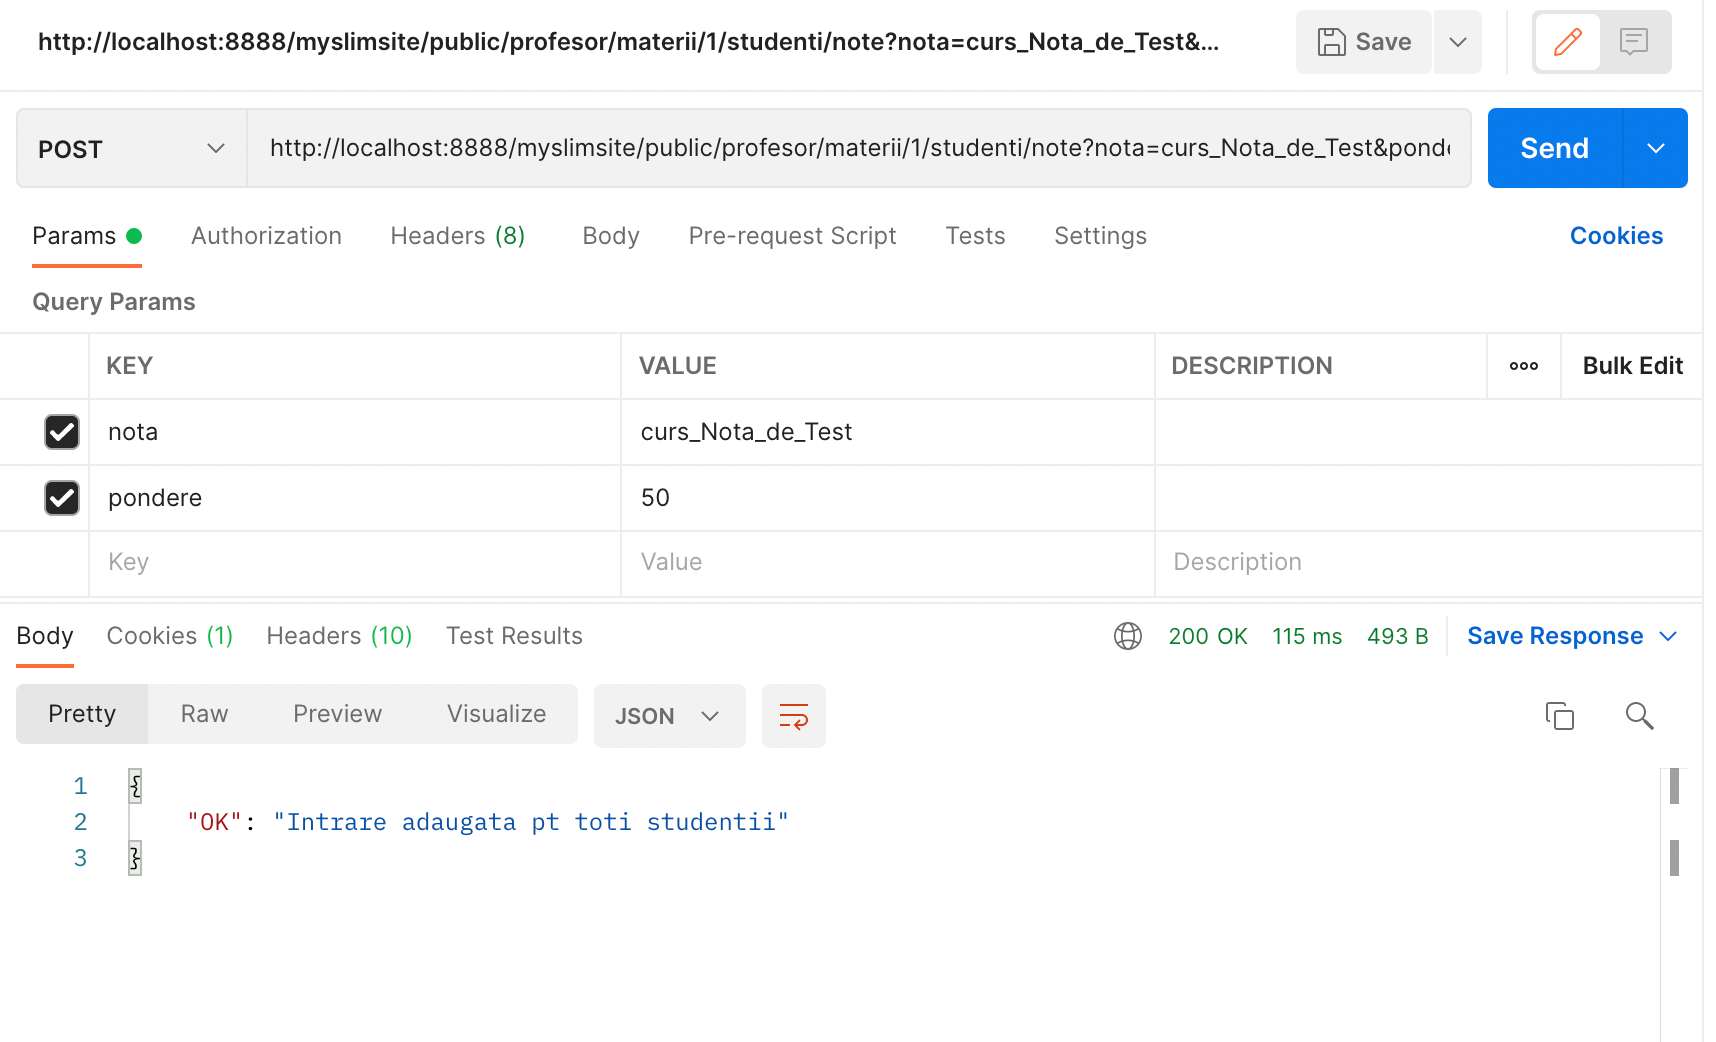
\includegraphics[width=300pt]{img/POST_OK.png}
    \caption{Testare cerere POST via Postman (success)}
    \label{POST_OK}
\end{figure}


Iar, dacă încercăm să adăugăm din nou aceea\c si notă, vom primi eroare, a\c sa cum sugerează figura \ref{POST_ERR}.

\begin{figure}[h!]
    \centering
    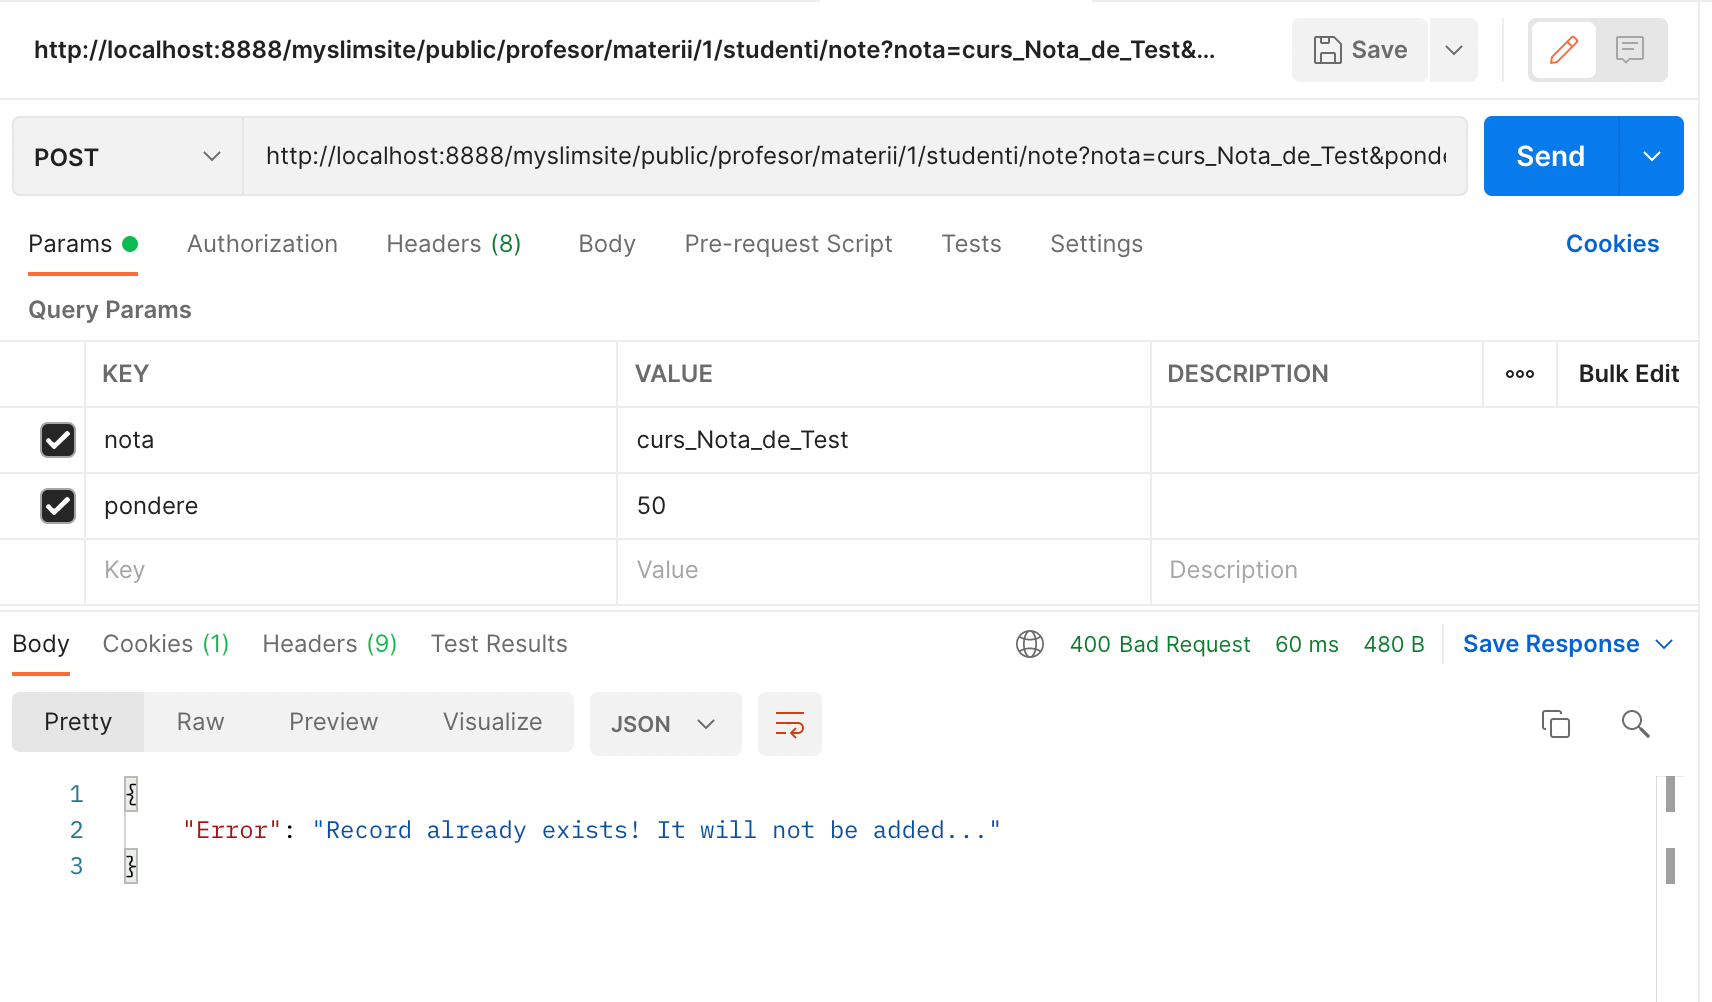
\includegraphics[width=300pt]{img/POST_ERR.png}
    \caption{Testare cerere POST via Postman (error)}
    \label{POST_ERR}
\end{figure}
\section{Cereri tip PUT}

Modificăm o anumită notă, la o anumită materie, pentru un anume student, a\c sa cum sugerează figura \ref{PUT_OK}.

\begin{figure}[h!]
    \centering
    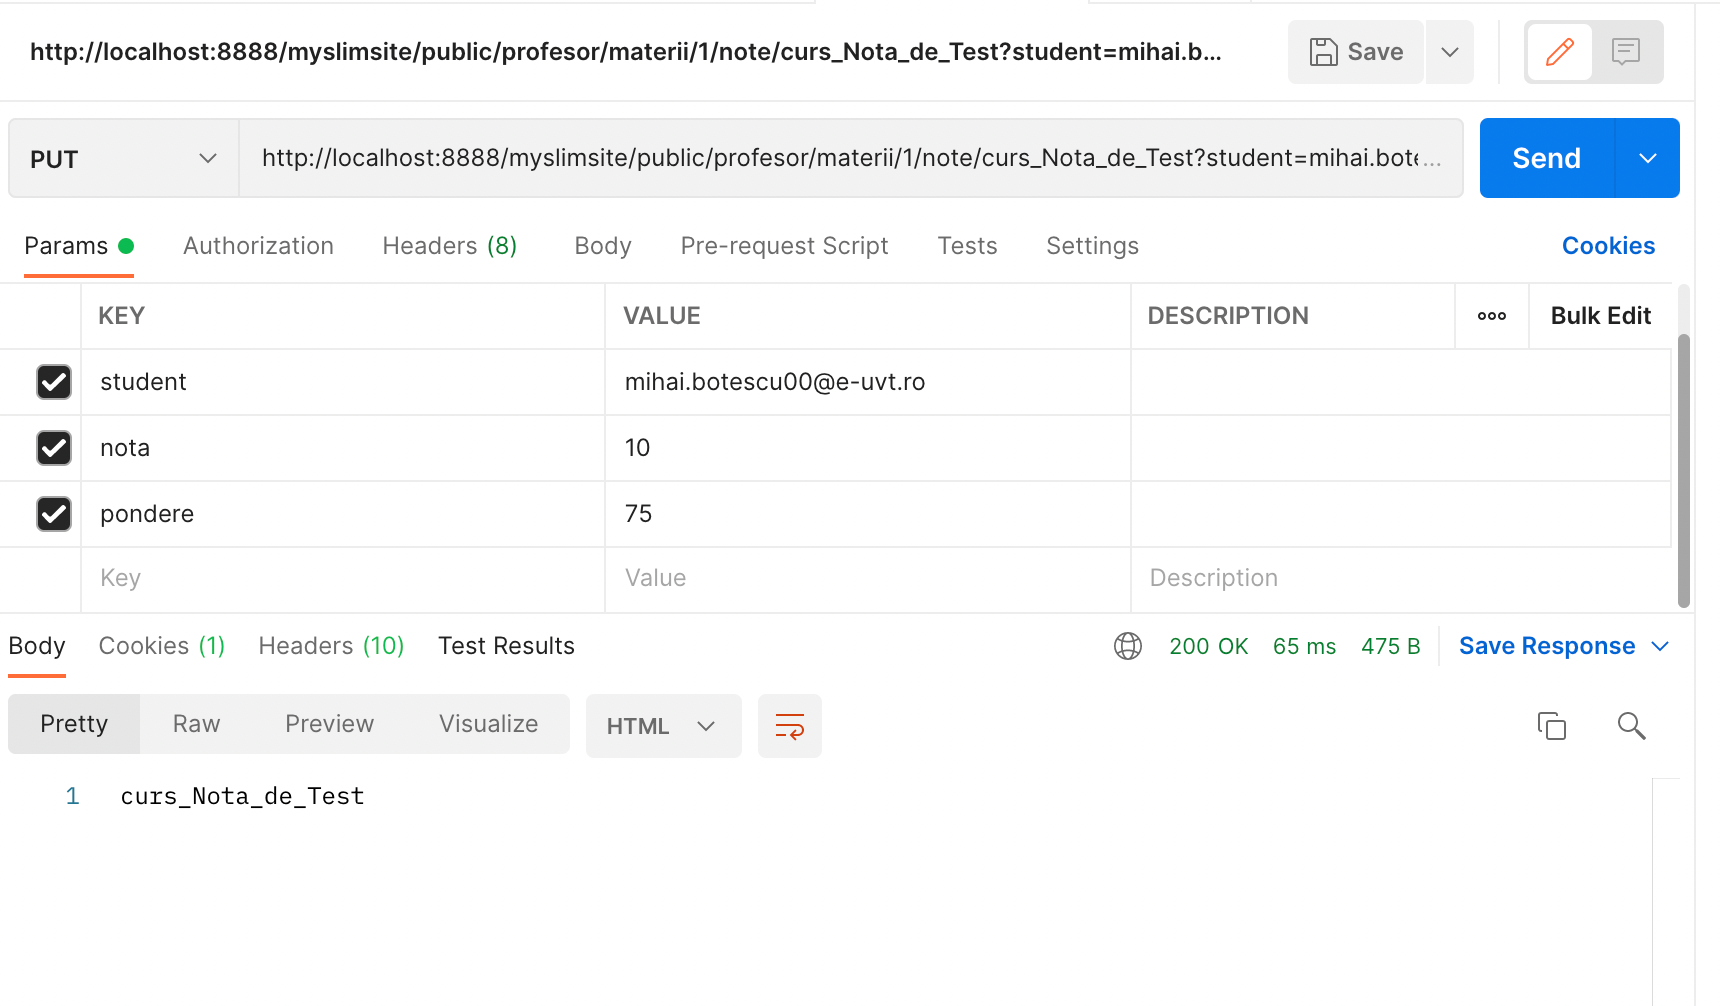
\includegraphics[width=300pt]{img/PUT_OK.png}
    \caption{Testare cerere PUT via Postman (success)}
    \label{PUT_OK}
\end{figure}

\section{Cereri tip DELETE}

\c stergem un anume tip de notă, de la o anumită materie, pentru to\c ti studen\c tii înscri\c si la aceasta, a\c sa cum sugerează figura \ref{DELETE_OK}.


\begin{figure}[h!]
    \centering
    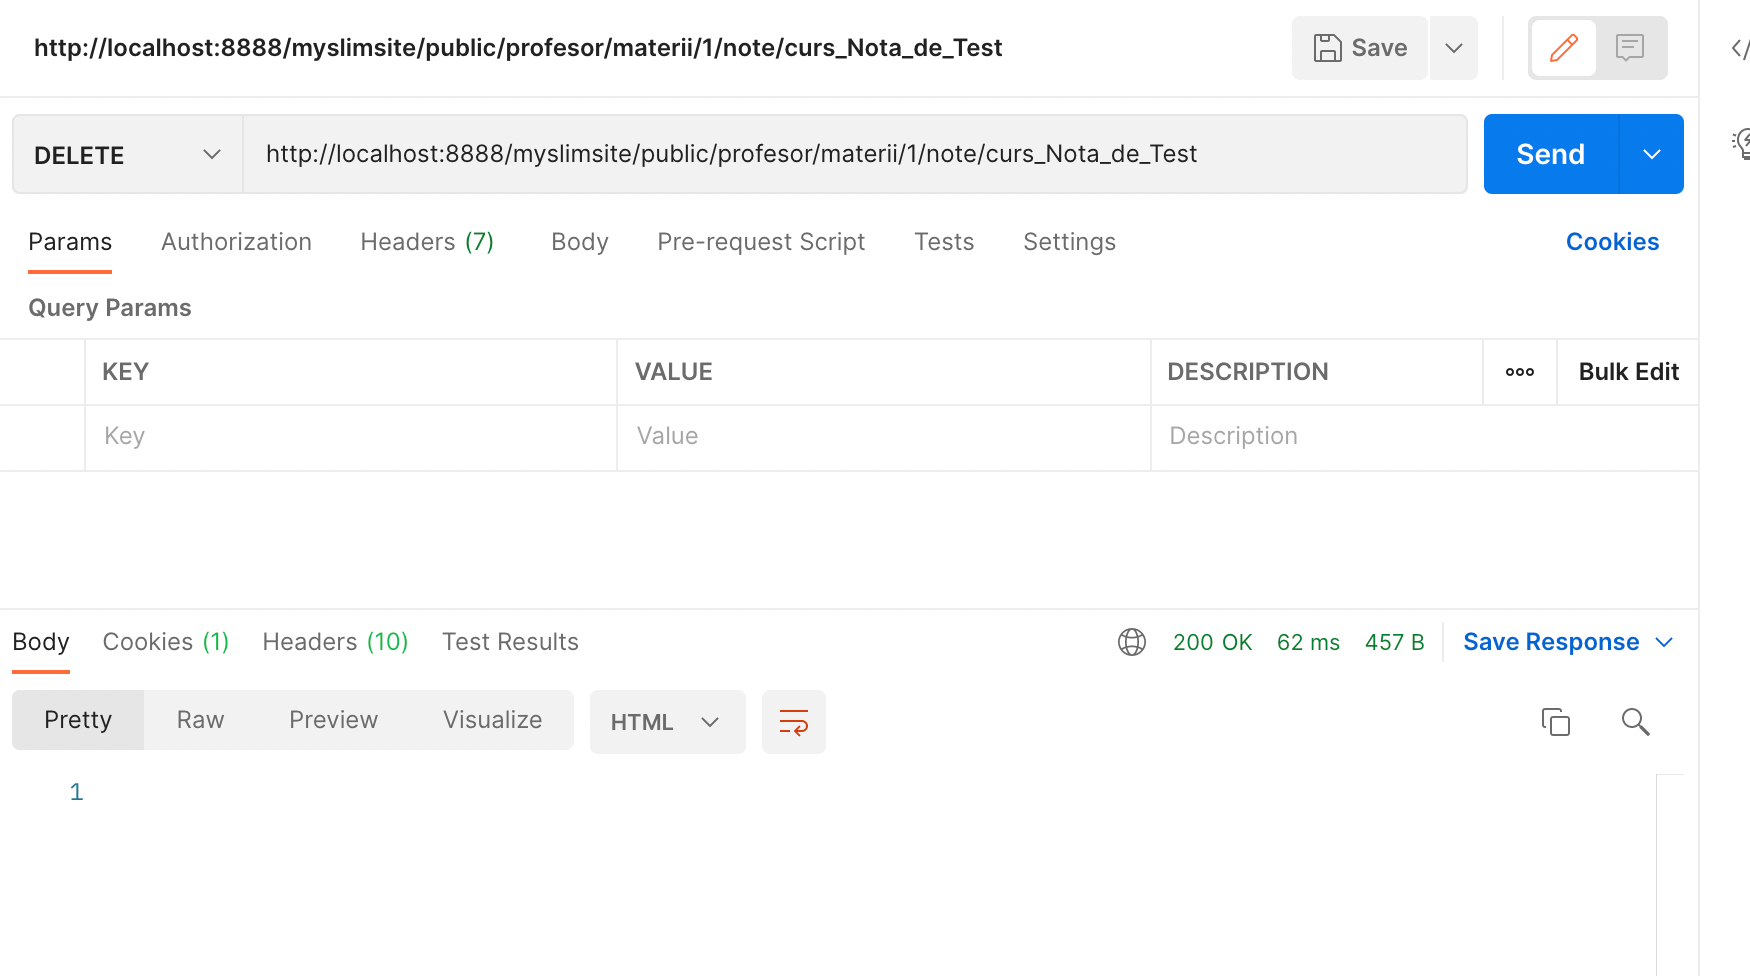
\includegraphics[width=300pt]{img/DELETE_OK.png}
    \caption{Testare cerere DELETE via Postman (success)}
    \label{DELETE_OK}
\end{figure}



\chapter{Concluzii \c si direc\c tii viitoare}

Ca \c si direc\c tii viitoare de realizare, se dore\c ste în primul rând extinderea aplica\c tiei spre utilizarea acesteia pe telefon mobil (deci creearea unui client iOS/Android care să poată consuma serviciile ReST expuse aici \c si să le uniformizeze în propria interfa\c tă). Mai apoi, pentru profesor, export-ul de date dintr-un fi\c sier CSV pentru înregistrarea studen\c tilor în aplica\c tie.

	\bibliography{mybib}
		\bibliographystyle{ieeetr}
		\addcontentsline{toc}{chapter}{Bibliografie}




\end{document}
